\documentclass{beamer}
\usetheme{Madrid}
\usepackage{graphicx}
\graphicspath{{figs/}}

\title{Role-Specialized Steering for Latent MAS}
\subtitle{Where does reasoning live in LatentMAS --- and what can we steer?}
\author{Sagnik Biswas}
\date{July 2026}

\begin{document}

\begin{frame}
    \titlepage
    \vspace{-1cm}
\end{frame}

\begin{frame}{Where We Started (and the advisor's ask)}
    \textbf{Established:} SEAL on the LatentMAS \textbf{Judger} cuts output tokens with accuracy retained.
    \vspace{0.2cm}
    \begin{block}{Advisor's next-step checklist}
        \begin{enumerate}
            \item Evaluate SEAL steering on Planner / Critic / Refiner / Judger \emph{separately}.
            \item For sub-agents where SEAL fails, develop \emph{new} steering-vector strategies.
            \begin{itemize}
                \item Plot execution vs non-execution thought ratios per sub-agent; explain why SEAL works or not.
                \item Propose new thought-type divisions for more effective sub-agent vectors.
            \end{itemize}
        \end{enumerate}
    \end{block}
    \textbf{This talk answers all three --- including an honest negative and the mechanism behind it.}
\end{frame}

\begin{frame}{Recap: Judger Steering Is a Clean Token Win}
    \textbf{SEAL vector at layer 28, applied to the Judger's decode (GSM8K, n=120)}
    \begin{table}[]
        \centering\small
        \begin{tabular}{|c|c|c|c|}
            \hline
            \textbf{coef} & \textbf{Accuracy} & \textbf{Mean tokens} & \textbf{$\Delta$ tokens} \\ \hline
            0 (control) & 93.3\% & 621 & --- \\ \hline
            40 & \textbf{95.0\%} & 515 & $-$17\% \\ \hline
            80 & 94.2\% & 379 & \textbf{$-$39\%} \\ \hline
        \end{tabular}
    \end{table}
    \begin{itemize}
        \item Monotonic; accuracy held or improved; $\sim$2$\times$ faster decode.
        \item Transfers: GSM8K vector $\rightarrow$ ARC-C gives $-$25\% tokens at identical accuracy.
    \end{itemize}
\end{frame}

\begin{frame}{Ask \#1: Per-Agent Steering --- Only the Judger Moves}
    \textbf{Same vector, one agent steered at a time (GSM8K, control 621 / 93.3\%)}
    \begin{table}[]
        \centering\small
        \begin{tabular}{|l|c|c|}
            \hline
            \textbf{Steered agent} & \textbf{coef 40} & \textbf{coef 80} \\ \hline
            \textbf{Judger} & 515 / 95.0\% & \textbf{379 / 94.2\%} \\ \hline
            Planner & 580 / 95.0\% & 593 / 94.2\% \\ \hline
            Critic & 635 / 94.2\% & 615 / 95.8\% \\ \hline
            Refiner & 623 / 91.7\% & 608 / 95.0\% \\ \hline
        \end{tabular}
    \end{table}
    \begin{center}\textit{Only Judger steering reduces tokens. Steering all agents $\approx$ Judger-only.}\end{center}
\end{frame}

\begin{frame}{Ask \#2a: Why? Thought Distribution Is Uniform}
    \textbf{Classify every reasoning step per role (GSM8K)}
    \begin{table}[]
        \centering\small
        \begin{tabular}{|l|c|c|}
            \hline
            \textbf{Role} & \textbf{execution} & \textbf{non-execution} \\ \hline
            Planner & 87.5\% & 12.5\% \\ \hline
            Critic & 87.8\% & 12.2\% \\ \hline
            Refiner & 88.8\% & 11.2\% \\ \hline
            Judger & 88.2\% & 11.8\% \\ \hline
        \end{tabular}
    \end{table}
    \begin{itemize}
        \item All four roles are $\sim$88\% execution --- \textbf{no distributional difference}.
        \item SEAL is a \textbf{length} lever; it only bites the Judger because the Judger is the \textbf{sole text-emitter}. The effect is \textbf{structural}, not about reflectiveness.
    \end{itemize}
\end{frame}

\begin{frame}{Ask \#2b: A New Strategy --- Correctness-Contrastive Vectors}
    \textbf{Sub-agents emit no text $\Rightarrow$ steer for \emph{quality}, not length.}
    \begin{itemize}
        \item New thought-division: instead of execution$-$reflection, use
        \[ v_{\text{agent}} = \text{mean(latent} \mid \text{correct)} - \text{mean(latent} \mid \text{incorrect)} \]
        \item Extracted \textbf{in-pipeline}, text-free, from each agent's real layer-28 latent state (conditioned on upstream KV), labeled by final answer correctness.
        \item Applied during each sub-agent's latent-thought generation; evaluated end-to-end.
    \end{itemize}
    \begin{center}\textit{This is a steering objective designed for latent agents, not ported from text.}\end{center}
\end{frame}

\begin{frame}{The Mechanism: Correctness Is Decided \emph{Late}}
    \textbf{Per-agent correctness probe (5-fold AUC of latent state $\rightarrow$ final correctness)}
    \begin{table}[]
        \centering\small
        \begin{tabular}{|l|c|c|c|}
            \hline
            \textbf{Agent (AUC $\uparrow$)} & \textbf{GSM8K} & \textbf{ARC-C} & \textbf{MedQA} \\ \hline
            Planner & 0.54 & 0.57 & 0.57 \\ \hline
            Critic & 0.62 & 0.51 & 0.63 \\ \hline
            Refiner & 0.59 & 0.46 & 0.64 \\ \hline
            \textbf{Judger} & \textbf{0.69} & \textbf{0.73} & \textbf{0.80} \\ \hline
        \end{tabular}
    \end{table}
    \begin{itemize}
        \item Outcome is barely linearly encoded upstream (0.46--0.64, near chance) but clearly decodable at the Judger (0.69--0.80).
        \item Also: wrong answers \textbf{over-generate by 70--82\%} --- length is coupled to failure \emph{at the Judger}.
    \end{itemize}
\end{frame}

\begin{frame}{Ask \#2b Result: Honest Negative}
    \textbf{Native/upstream steering vs Judger-only SEAL (GSM8K test, n=300; control 92.7\% / 602 tok)}
    \begin{table}[]
        \centering\small
        \begin{tabular}{|l|c|c|c|}
            \hline
            \textbf{Steering} & \textbf{coef} & \textbf{Acc} & \textbf{Tokens} \\ \hline
            control & 0 & 92.7\% & 602 \\ \hline
            Critic (native) & 40 & 92.7\% & 586 \\ \hline
            Upstream-3 (native) & 80 & 93.3\% & 608 \\ \hline
            Judger (native) & 80 & 91.0\% & 658 \\ \hline
            \textbf{Judger (generic SEAL)} & 80 & 93.0\% & \textbf{390 ($-$35\%)} \\ \hline
        \end{tabular}
    \end{table}
    \begin{itemize}
        \item Upstream steering: within noise, \textbf{no token savings}; hurts MedQA.
        \item As the probe predicted --- steering fixed upstream agents can't smooth a late-decided outcome.
    \end{itemize}
\end{frame}

\begin{frame}{Also Explored: KV Cache Steering of the Handoff}
    \textbf{New mechanism (arXiv:2507.08799): steer the KV cache the Judger reads.}
    \begin{center}
        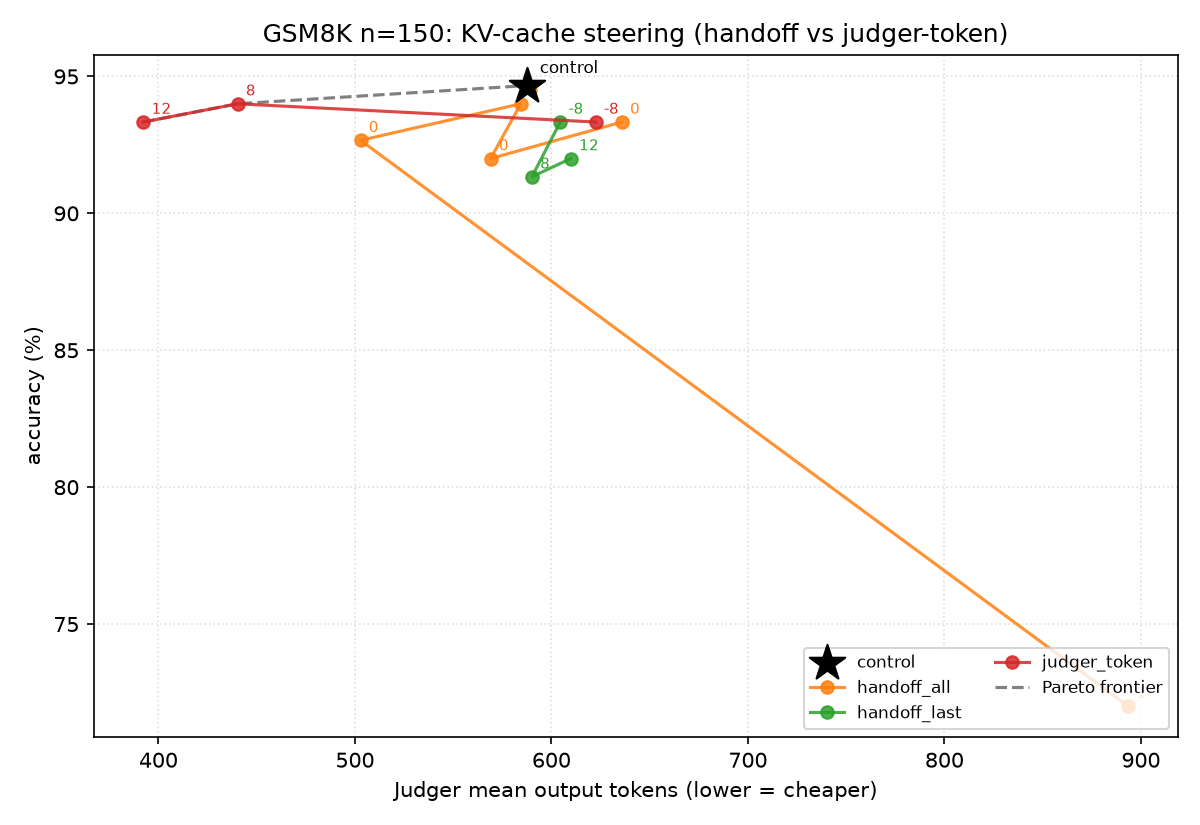
\includegraphics[width=0.62\textwidth]{kv_gsm8k.png}
    \end{center}
    \vspace{-0.2cm}
    \begin{itemize}
        \item Steering the latent \textbf{handoff}: no gain, destructive at strength (attention saturation).
        \item Steering the \textbf{Judger's own token}: $-$25\% to $-$33\% tokens, accuracy held --- same lesson, third method.
    \end{itemize}
\end{frame}

\begin{frame}{Methodology Check (due diligence)}
    \textbf{We stress-tested our own surprising results against the source paper.}
    \begin{itemize}
        \item LatentMAS' method uses a realignment matrix $W_a$ (hidden $\rightarrow$ input-embedding) --- our default runs had it \textbf{off}; MedQA was capped at 2048 vs the paper's 4096.
        \item Re-running the faithful config (with $W_a$, 4096) to confirm the base scaffold reproduces the paper's gains before drawing scaffold-level conclusions.
    \end{itemize}
    \vspace{0.2cm}
    \begin{center}\textit{Catching this before believing a contrarian result --- not after.}\end{center}
\end{frame}

\begin{frame}{Synthesis: Where Reasoning Lives}
    \begin{center}
        \Large \textbf{Core Finding} \\
        \vspace{0.4cm}
        \normalsize
        In sequential latent MAS, the \textbf{decision is localized at the text-emitting Judger}. Three independent steering methods (SEAL residual, correctness-contrastive native, KV-cache) all converge: \textbf{the Judger is the only effective intervention point}; upstream latent steering does not move the accuracy--token frontier, and the correctness probe explains why.
    \end{center}
\end{frame}

\begin{frame}{What's the Contribution (two viable framings)}
    \begin{enumerate}
        \item \textbf{Analysis / localization paper (strongest given evidence):}
        ``Where is reasoning localized in latent MAS, and what does it imply for steering?'' --- per-agent steering + thought distributions + correctness-probe AUC + three converging steering methods. A principled account of why upstream steering fails.
        \item \textbf{Method paper:} one-shot Judger cache/residual steering for token-efficient latent MAS ($-$25 to $-$39\% tokens, accuracy held, transfers).
    \end{enumerate}
    \vspace{0.2cm}
    \textit{Open for discussion: is a positive sub-agent steering result reachable, or is the localization result itself the contribution?}
\end{frame}

\begin{frame}{Limitations \& Next Steps}
    \textbf{Limitations}
    \begin{itemize}
        \item n = 100--300, 1--2 seeds; single backbone (Qwen3-14B), single layer (28).
        \item Class imbalance in native-vector capture (few negatives on easy tasks).
    \end{itemize}
    \vspace{0.1cm}
    \textbf{Next steps}
    \begin{itemize}
        \item Confirm base scaffold with $W_a$ on (running now); n$\geq$500 multi-seed for the frontier.
        \item If pursuing sub-agent steering: try the \textbf{hierarchical} topology (where sub-agents may carry more outcome signal) and non-linear / process-level objectives.
        \item Otherwise: commit to the localization analysis as the contribution.
    \end{itemize}
\end{frame}

\end{document}
